% ---------------------------------------------------------------- 05-extensions.tex
\section{Extensions}\label{sec:ext}

The base model rests on four simplifications that could overturn its conclusion. Each extension below relaxes one of them; Appendix~\ref{app:C} reports the detailed results.

\subsection{Market-priced debt}\label{sec:mkt}

The base model holds the borrowing rate at 10\% regardless of leverage, so lenders implicitly accept losses once default becomes possible. We now require lenders to break even: the promised repayment $F$ solves $D = \Ex[\text{payoff to creditors}]/(1 + r)$, and the full coupon $F - D$ is deductible. In the lognormal model the break-even rate is 10.4\% at the optimum ($D \approx 35$), 13.8\% at $D = 45$, 19.3\% at $D = 50$ and 32.5\% at $D = 55$ (Figure~\ref{fig:C1}b, Appendix~\ref{app:C}). The optimal debt level and the maximum gain are almost unchanged ($D = 35$ and 0.57, against 34 and 0.56).

What changes is the allocation of distress costs (Figure~\ref{fig:C1}a). Under a fixed rate, shareholders gain $\VL - \VU$ plus the lenders' loss, a quantity that rises with debt (2.1 at $D = 50$ and 5.1 at $D = 60$), so they would choose leverage far above the value-maximising level. With fair pricing, expected distress costs are borne by shareholders through the interest rate, and maximising shareholder wealth coincides with maximising $\VL$. The fixed-rate assumption is thus innocuous for firm value but distorts incentives, which is why lenders rely on covenants, ratings and credit spreads. This is the agency conflict that Lecture~1 (p.~50) lists among the costs of debt: at $D = 50$, shareholders who borrow at a rate that ignores default risk gain 2.06 while the firm as a whole loses 0.66 (Table~\ref{tab:C2}).

\subsection{Usability of the interest deduction}\label{sec:usable}

Because the base firm always earns at least 60, every unit of interest reduces tax. Actual firms have loss years, and many tax codes cap interest deductions; the United States, for example, limits net interest to 30\% of adjusted taxable income (Section~\ref{sec:tcja}). We draw EBIT from a normal distribution with a given volatility (standard deviation over mean) and compute the share of $\tauc \times \text{interest}$ that is actually saved as a function of interest coverage, $\Ex[\text{EBIT}]/\text{interest}$ (Figure~\ref{fig:usable}a). Our firm, with volatility 0.28 and coverage of about 20 at $D = 44$, uses essentially all of its shield. A cyclical firm with volatility 1.0 loses about 17\% of its shield even at a coverage of 10, because of loss years. A 30\%-of-EBIT cap binds in an average year once coverage falls below 3.3 (and in bad years even above it); at a coverage of 2 only about 60\% of the shield is usable. The effective tax rate on interest is therefore below the statutory rate, and most so when leverage is high, which adds a tax-side limit to debt alongside distress costs \citep{deangelo1980}.

\subsection{Personal taxes}\label{sec:personal}

If lenders pay tax $\tauD$ on interest and shareholders pay $\tauE$ on equity income, the net tax advantage of one unit of interest is \citep{miller1977}
\begin{equation}
  \Tstar = 1 - \frac{(1 - \tauc)(1 - \tauE)}{1 - \tauD},
  \label{eq:miller}
\end{equation}
which equals $\tauc$ only when $\tauD = \tauE$. Table~\ref{tab:personal} shows that investor-level taxes can matter as much as the corporate rate. For a top-bracket US individual the net advantage was 12.5\% before the 2017 reform and is slightly negative afterwards, whereas for a tax-exempt investor it simply equals $\tauc$. Whether debt offers any tax advantage at all therefore depends on the identity of the marginal investor.

\begin{table}[htbp]\centering\footnotesize
\caption{Net tax advantage of debt per unit of interest, $\Tstar$}\label{tab:personal}
\begin{tabularx}{\linewidth}{@{}>{\raggedright\arraybackslash}p{6.6cm}CCCC@{}}
\toprule
Setting & $\tauc$ & $\tauD$ (interest) & $\tauE$ (equity) & $\Tstar$ \\
\midrule
Base model (no personal taxes) & 20\% & 0\% & 0\% & 20.0\% \\
United States 2017, top-bracket individual & 35\% & 43.4\% & 23.8\% & 12.5\% \\
United States from 2018, top-bracket individual & 21\% & 40.8\% & 23.8\% & $-1.7\%$ \\
United States, tax-exempt investor (2017 $\to$ 2018) & 35\% $\to$ 21\% & 0\% & 0\% & 35\% $\to$ 21\% \\
Singapore, individual investor & 17\% & 0\% & 0\% & 17.0\% \\
S-REIT distributing its income & $\approx 0\%$ & 0\% & 0\% & $\approx 0\%$ \\
\bottomrule
\end{tabularx}
\tablenote{\textit{Notes:} US rates are top federal statutory rates including the 3.8\% net investment income tax; deferral of capital gains would lower the effective $\tauE$ further. Sources are given in Section~\ref{sec:apps}.}
\end{table}

\subsection{Multi-period debt}\label{sec:multi}

One-period debt generates a shield for one year only. If the same debt is maintained for $T$ years, the shield is worth
\begin{equation}
  \mathrm{PV}(\text{shield}) = \tauc D\bigl[1 - (1 + r)^{-T}\bigr],
  \label{eq:pvshield}
\end{equation}
which equals 0.73 for one year, 3.03 for five, 4.92 for ten and $\tauc D = 8.0$ for perpetual debt, the result of \citet{mm1963}. To compare like with like, we model a perpetual firm with the same annual EBIT distribution ($\VU = 720$) that issues perpetual debt and defaults in the first year in which EBIT falls short of interest, losing a fraction $c$ of its value. With annual default probability $p$, Appendix~\ref{app:B} shows that
\begin{equation}
  \VL - \VU = \frac{(1 - p)\tauc r D - p c \VU}{r + p}.
  \label{eq:perp}
\end{equation}

The trade-off survives, but the gain is an order of magnitude larger (Figure~\ref{fig:usable}b): the optimum is at $D/\VU = 57\%$, with interest coverage of 2.2 and an annual default probability of 0.3\%, and it adds 10.4\% to firm value. Doubling EBIT volatility lowers optimal leverage to 27\% and the gain to 4.5\%. The one-period horizon therefore understates the magnitude of the gain. For comparison, \citet{graham2000} estimates the gross tax benefit of debt at 9.7\% of firm value (4.3\% net of personal taxes); in our model the gross shield at the optimum is 11.1\%, of which 10.4\% remains after expected distress costs.

\begin{figure}[htbp]\centering
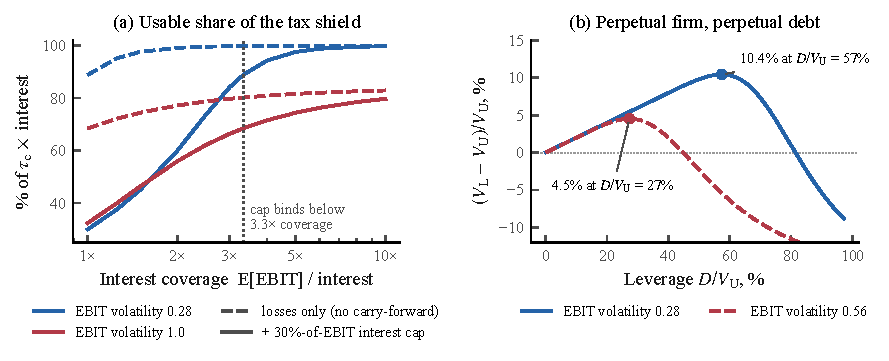
\includegraphics[width=15.2cm]{fig3_shield_multiperiod}
\caption{(a) Share of the statutory tax shield that is used, by interest coverage, for normally distributed EBIT with volatility (standard deviation over mean) of 0.28 or 1.0. Dashed lines allow for loss years only; solid lines add a 30\%-of-EBIT interest cap. (b) Perpetual firm with perpetual debt: value gain against leverage for lognormal EBIT with volatility 0.28 and 0.56.}\label{fig:usable}
\end{figure}
